


\documentclass{beamer}
\usetheme{Oxygen}
\usepackage{graphicx}

\title{\small Desarrollo de un prototipo de robot humanoide que busque, encuentre y patee
una pelota de forma aut\'onoma e inteligente}
\author{Jennifer Dos Reis y Juliana Le\'{o}n \linebreak Tutor Acad\'emico \linebreak Carolina Chang y Carolina Mart\'inez }
\begin{document}
\fontfamily{tahoma}
\frame{\titlepage}

\section*{}
\begin{frame}
  \frametitle{\'{I}ndice}
  \tableofcontents[section=1,hidesubsections]
\end{frame}

\AtBeginSection[]
{
  \frame<handout:0>
  {
    \frametitle{\'{I}ndice}
    \tableofcontents[currentsection,hideallsubsections]
	  }
}

\AtBeginSubsection[]
{
  \frame<handout:0>
  {
    \frametitle{\'{I}ndice}
    \tableofcontents[sectionstyle=show/hide,subsectionstyle=show/shaded/hide]
  }
}

\newcommand<>{\highlighton}[1]{%
  \alt#2{\structure{#1}}{{#1}}
}

\newcommand{\icon}[1]{\pgfimage[height=1em]{#1}}

\section{Introducci\'{o}n}

\begin{frame}
  \frametitle{Introducci\'{o}n}
  \begin{block}{}
  \begin{itemize}
    \item Futuro de la rob\'otica 
    \item Algunos ejemplos
    \item Competencia Robocup
  \end{itemize}
  \end{block}

\begin{figure}

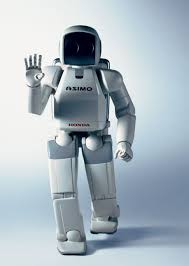
\includegraphics[scale=0.3]{asimo.jpg} 
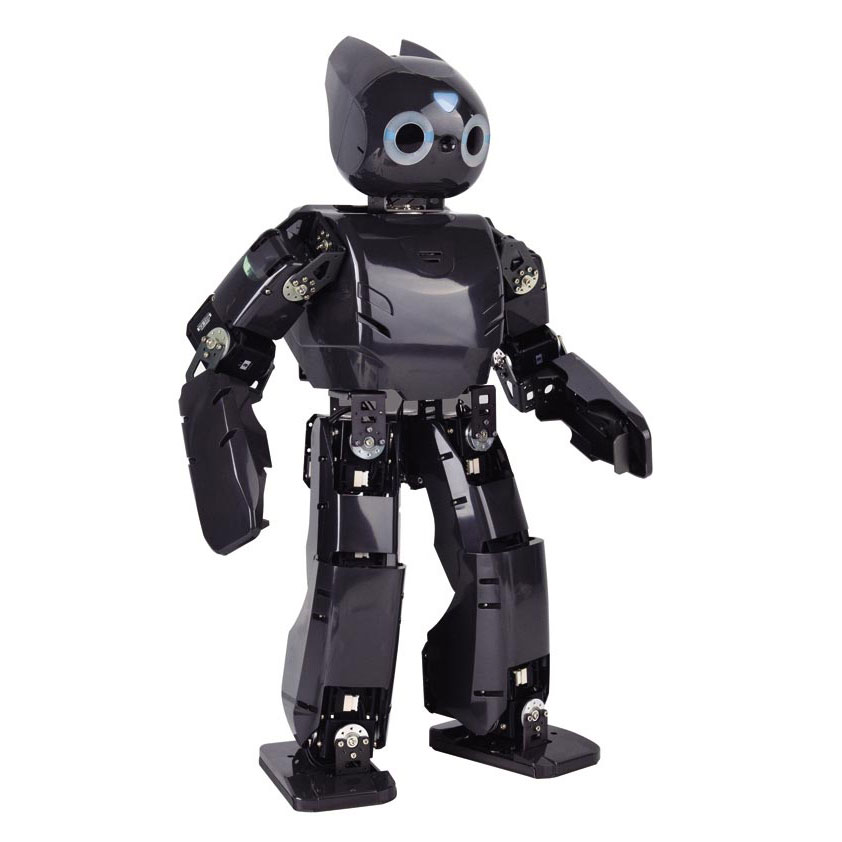
\includegraphics[scale=0.1]{Darwin_OP.jpg} 
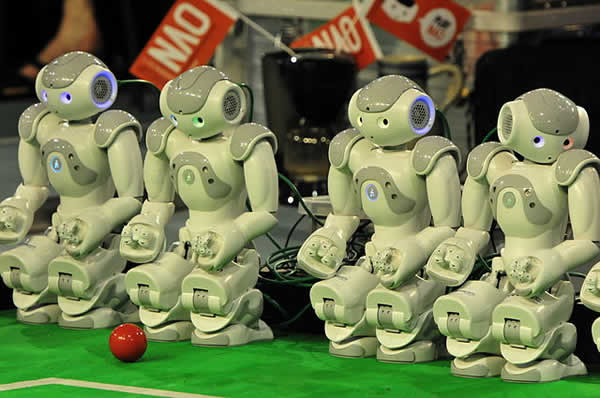
\includegraphics[scale=0.5]{13-06-28-robocup-eindhoven.jpg} 

\end{figure}
\end{frame}


\begin{frame}
  \frametitle{Introducci\'{o}n}
  \framesubtitle{Objetivo General}

  \begin{block}{Objetivo General}
	Dise\~nar y construir un robot humanoide capaz de detectar una pelota, buscarla y patearla con direcci\'on al arco, de forma aut\'onoma e inteligente.
   \end{block}
\end{frame}
\begin{frame}
  \frametitle{Introducci\'{o}n}
  \framesubtitle{Objetivos Espec\'{i}ficos}
  \begin{block}{Objetivos Espec\'{i}ficos}
  \begin{itemize}
    \item Dise\~no y ensamblaje
    \item Instalaci\'on y configuraci\'on de los componentes 
    \item Detecci\'on de la pelota
    \item Desplazamiento 
    \item Control de ca\'idas
    \item Comunicaci\'on entre controladores
    \item Aprendizaje por reforzamiento 
    \item Orientaci\'on al arco 
    \end{itemize}
  \end{block}
\end{frame}


  

\section{Construci\'on }
\begin{frame}
  \frametitle{Partes del robot}
  \framesubtitle{Piezas}

\begin{block}{Estructura}
	\begin{itemize}
		\item Con piezas de LEGO
		\item Desde cero
		\item Con el kit de piezas Bioloid
	\end{itemize}
\end{block}

 
\end{frame}

\begin{frame}
 \frametitle{Partes del robot}
 \framesubtitle{Piezas}
 
\begin{block}{Componentes utilizados del kit Bioloid}
\begin{itemize}
\item Motores Dynamixel
\item Bater\'ia de pol\'imero de litio
\item Giroscopio 
\end{itemize}
\end{block}

\begin{figure}[hbtp]
\centering
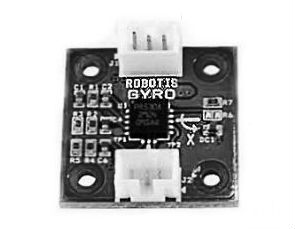
\includegraphics[scale=0.3]{gyro.jpg} 
\end{figure}

\end{frame}

\begin{frame}
 \frametitle{Partes del robot}
 \framesubtitle{Piezas}
 
\begin{block}{Componentes adicionales}
\begin{itemize}
\item Tarjeta controladora Arbotix
\item Raspberry Pi
\item C\'amara
\item Micro servo motores 
\item chip FTDI
\end{itemize}
\end{block}
\end{frame}

\begin{frame}
\frametitle{Partes del robot}
 \framesubtitle{Arbotix}
\centering
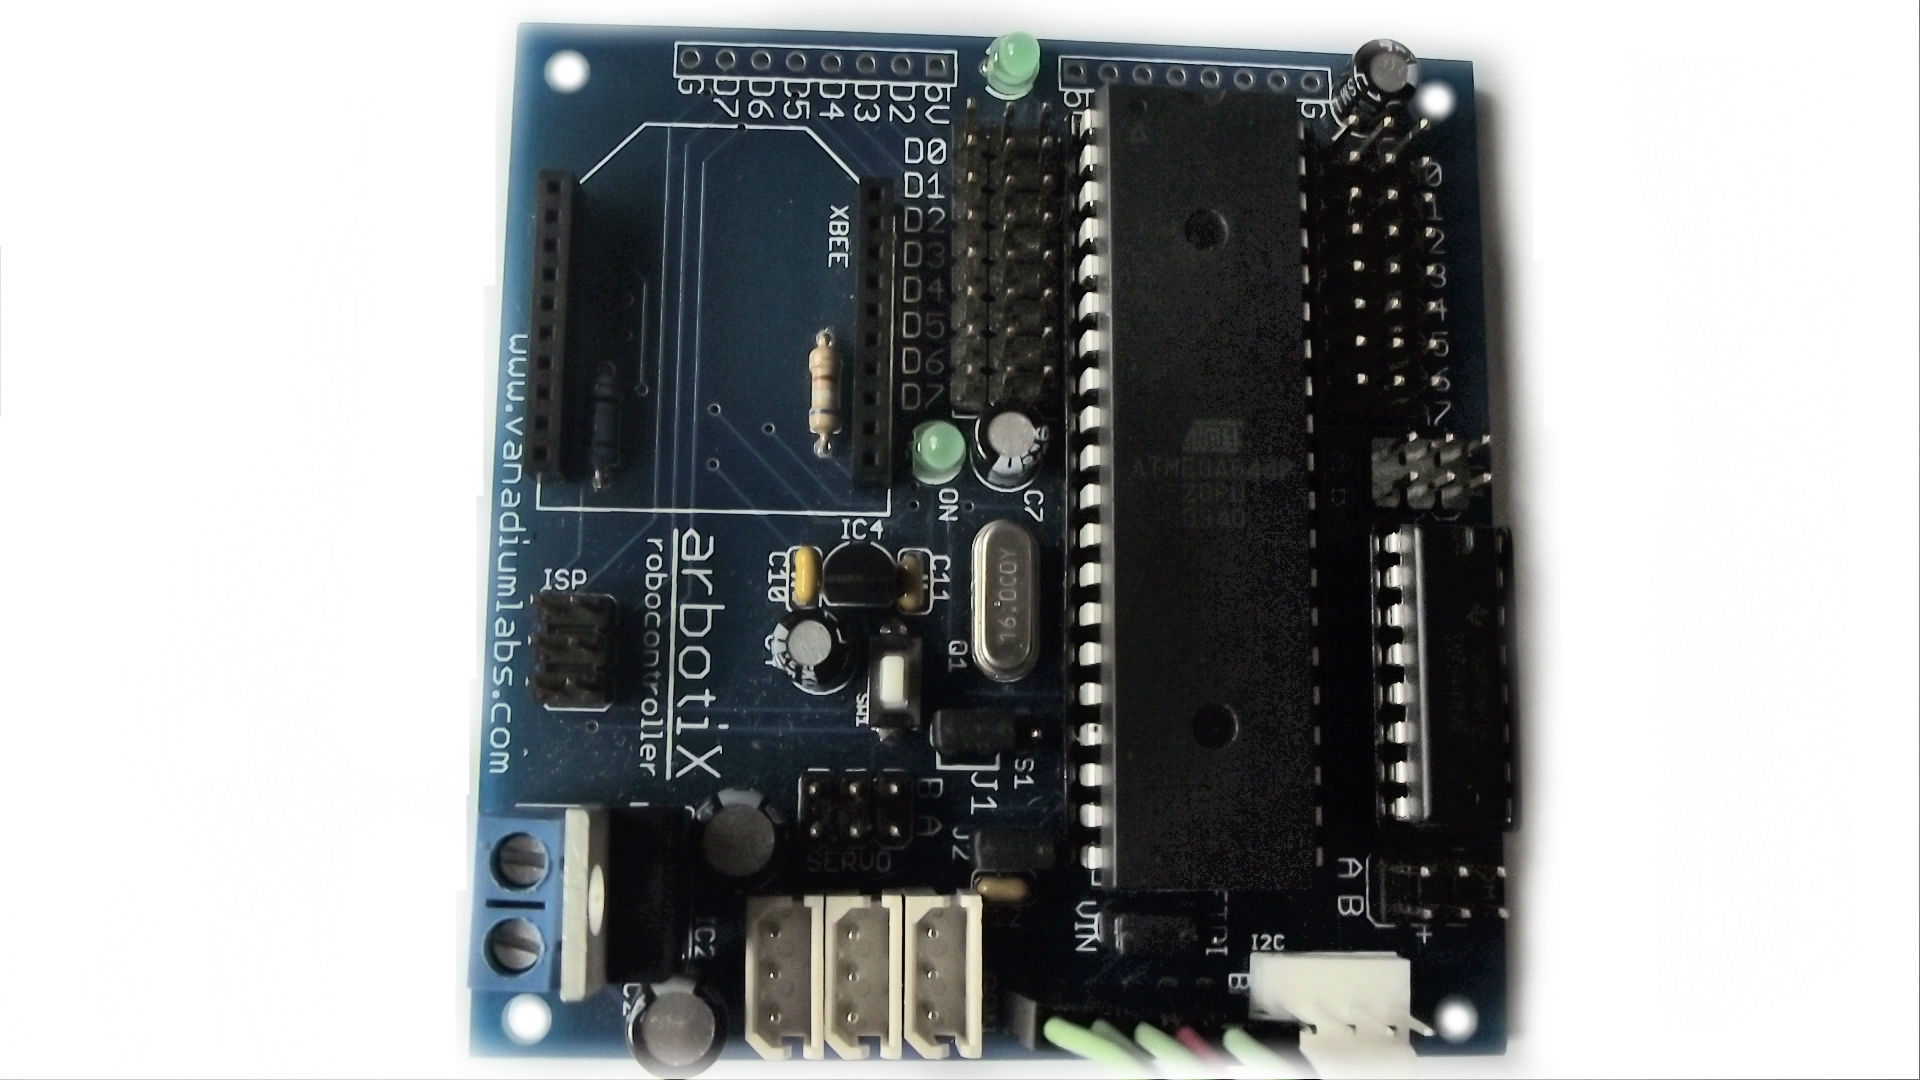
\includegraphics[scale=0.12]{Arbotix.jpg} 

\end{frame}

\begin{frame}
\frametitle{Partes del robot}
\framesubtitle{Ensamblaje}

\begin{block}{Modelo del robot}
	\begin{itemize}
		\item Modelo tipo B del manual	
	\end{itemize}
\end{block}

%\begin{block}{Desplazamiento}
%	\begin{itemize}
%	\item Escenas
%	\item Personal
%	\item Locaci\'{o}n
%\end{itemize}		
%\end{block}
\end{frame}

\begin{frame}
\frametitle{Partes del robot}
\framesubtitle{Conexiones}

%\begin{block}{Modelo del robot}
%	\begin{itemize}
%		\item Modelo tipo B del manual	
%	\end{itemize}
%\end{block}

\begin{figure}[hbtp]
\centering
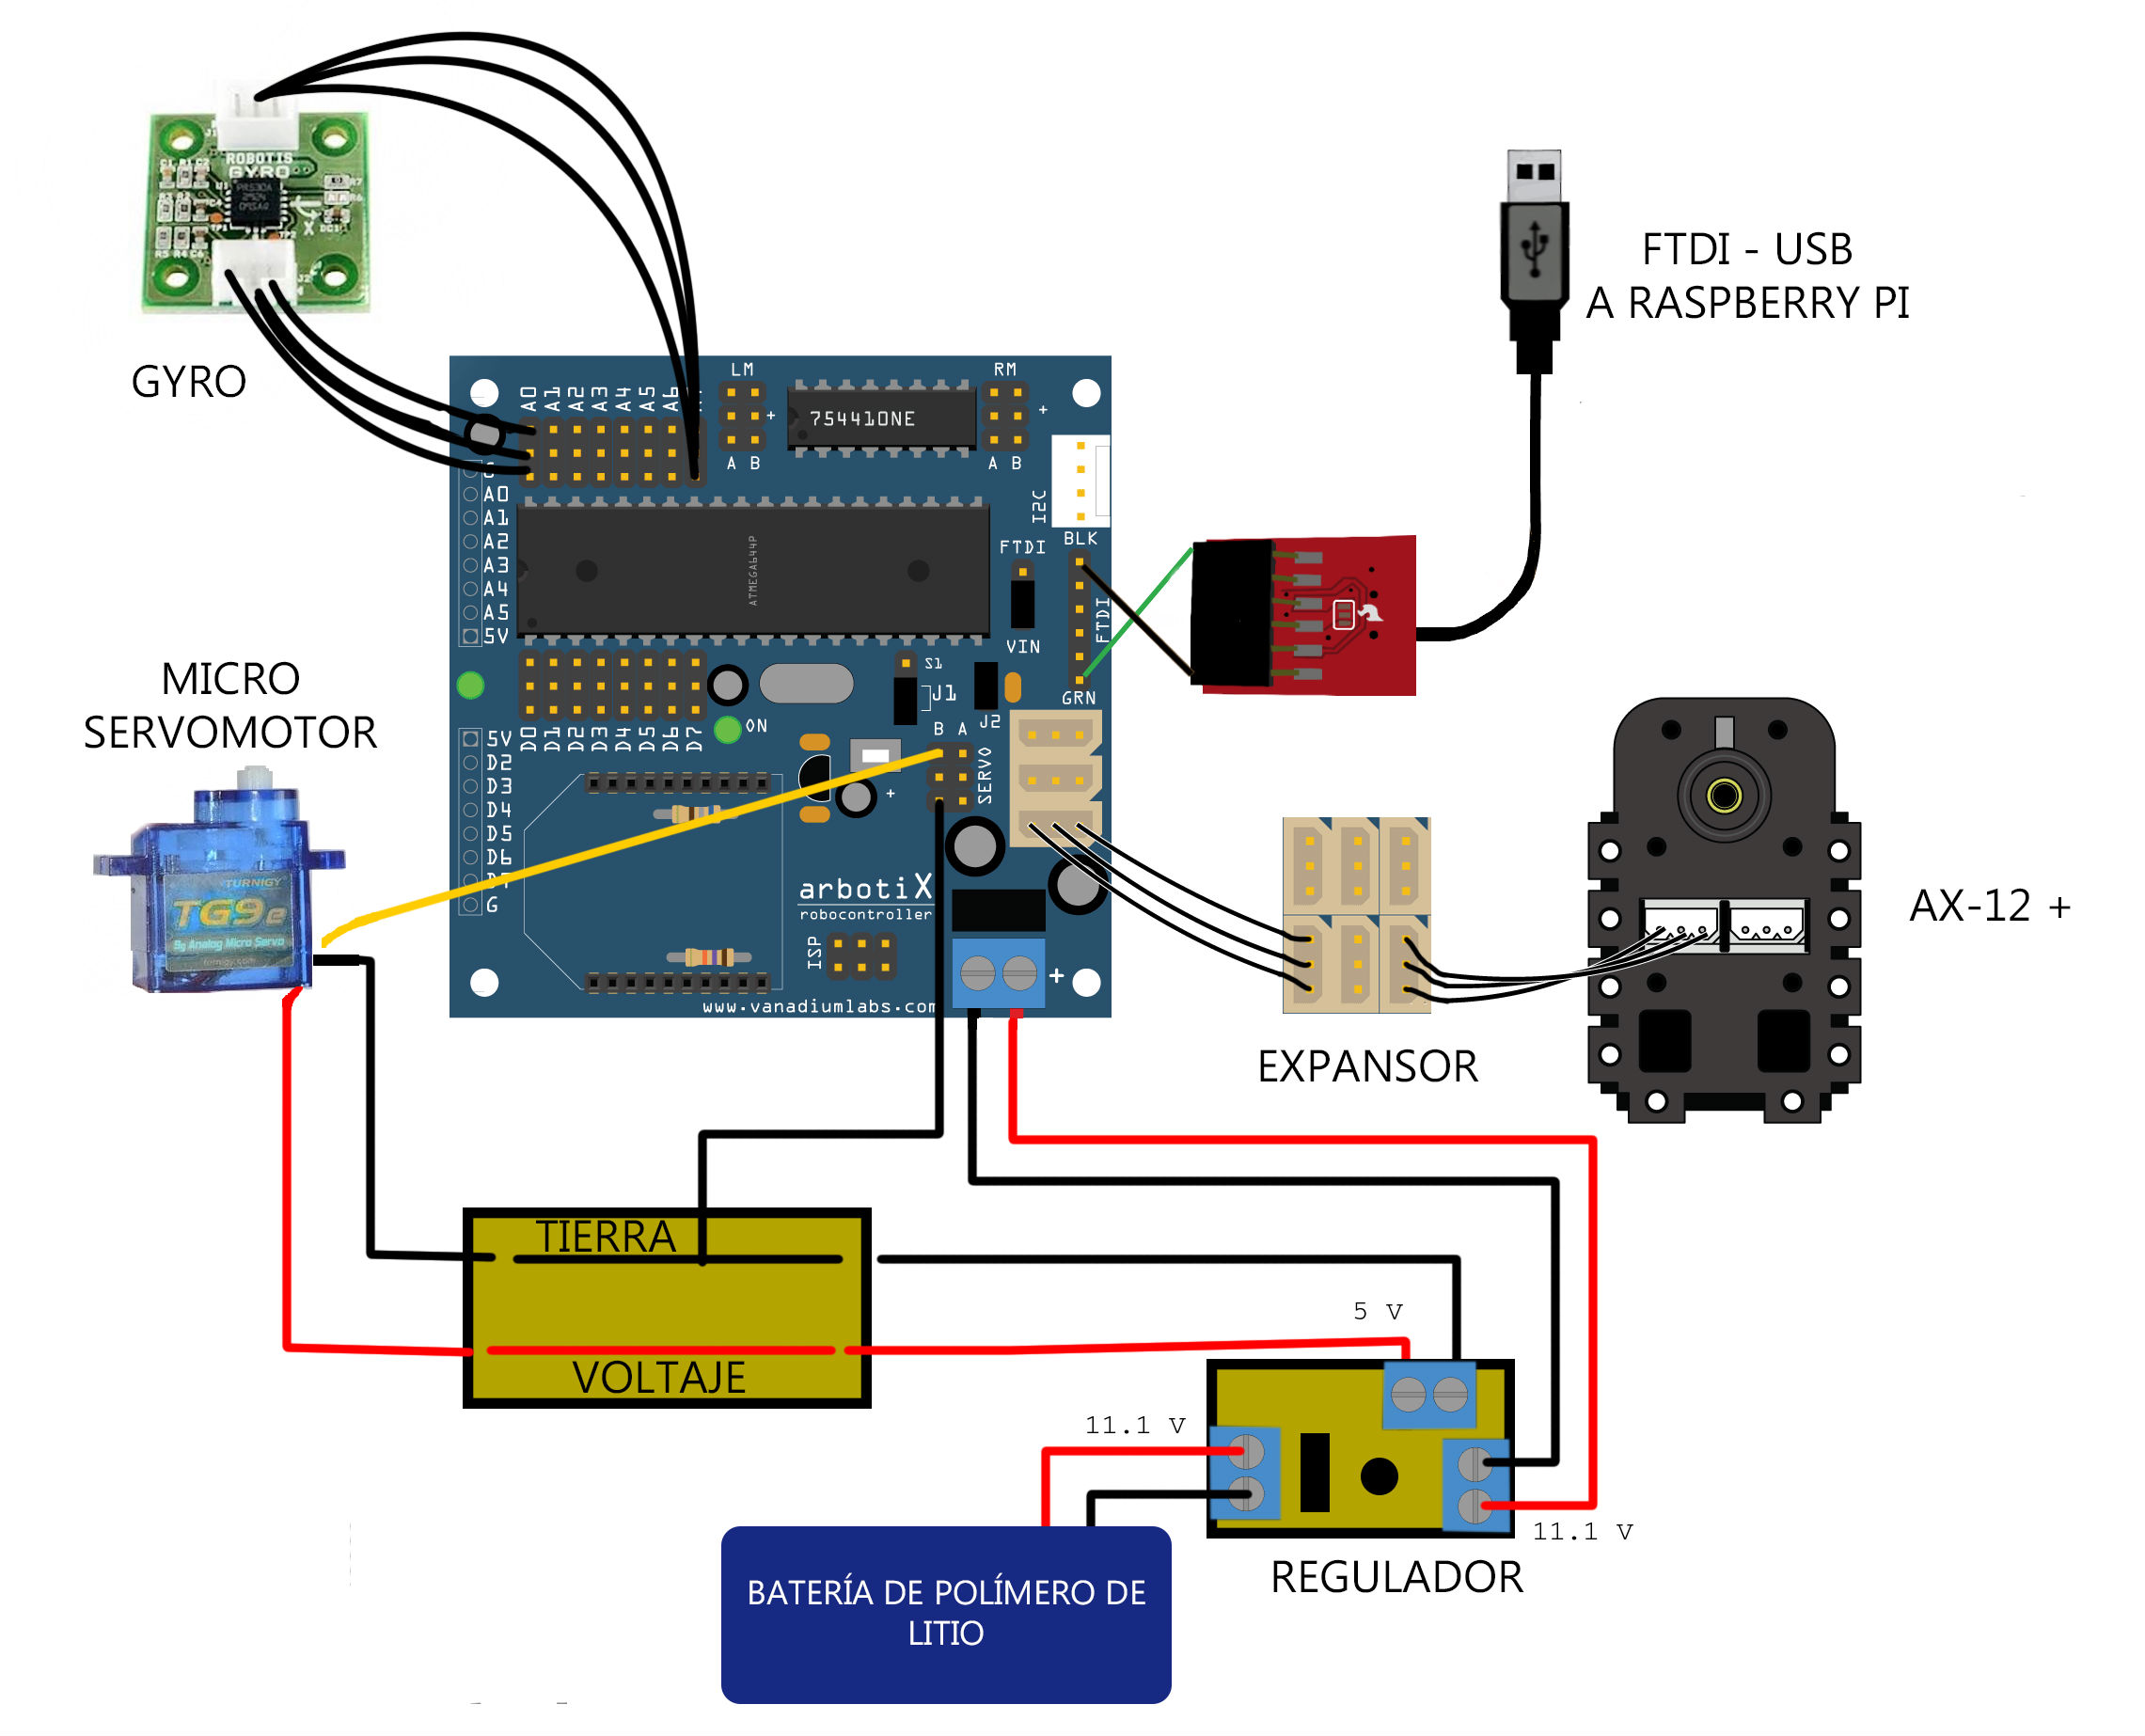
\includegraphics[scale=0.1]{arbotix_servo.jpg} 
\end{figure}

%\begin{block}{Desplazamiento}
%	\begin{itemize}
%	\item Escenas
%	\item Personal
%	\item Locaci\'{o}n
%\end{itemize}		
%\end{block}
\end{frame}

\begin{frame}
\frametitle{Detecci\'on de la pelota}

\begin{block}{Obtenci\'on de la imagen}
	\begin{itemize}
		\item Dificultades
		\item Soluci\'on	
	\end{itemize}
\end{block}

\begin{block}{Procesamiento de la imagen}
	\begin{itemize}
	\item De BGR a HSV
	\item Segmentaci\'on de regiones por color
	\item Filtros 
    \end{itemize}		
\end{block}

\end{frame}

\begin{frame}
\frametitle{Detecci\'on de la pelota}
\framesubtitle{Filtros: Ejemplo 1}

\begin{figure}[hbtp]
\centering
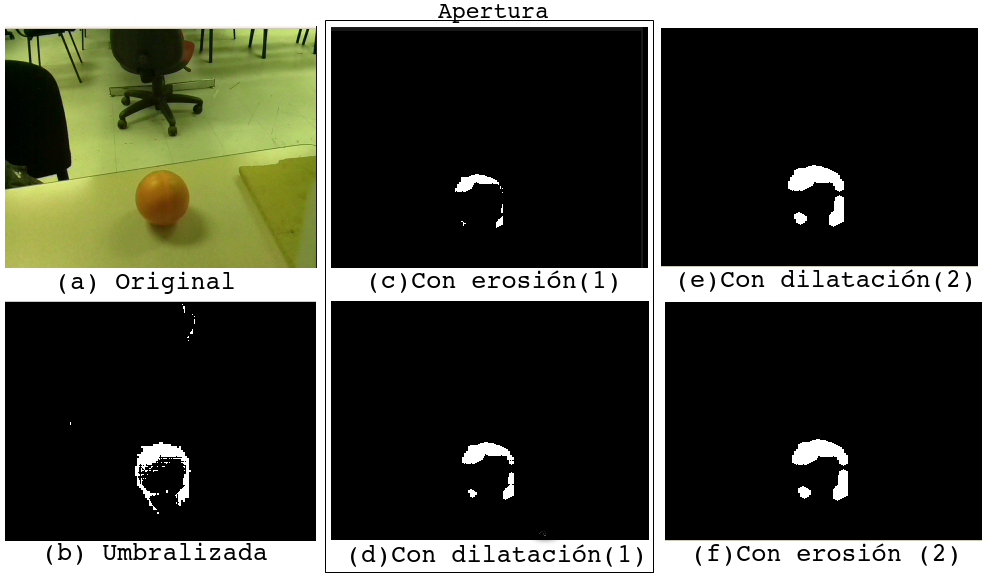
\includegraphics[scale=0.3]{filtros.png} 
\end{figure}

\end{frame}

\begin{frame}
\frametitle{Detecci\'on de la pelota}
\framesubtitle{Filtros: Ejemplo 2}

\begin{figure}[hbtp]
\centering
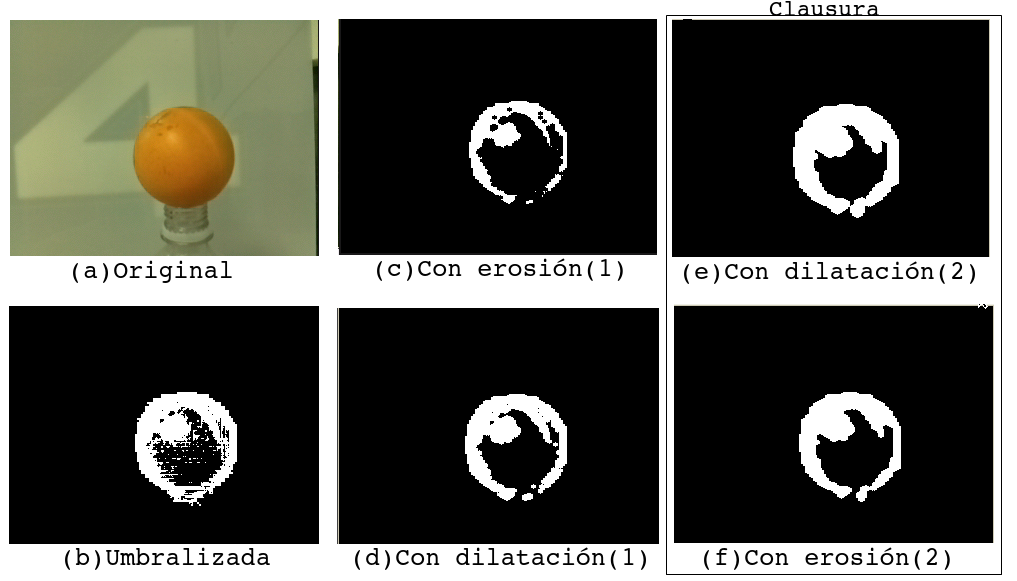
\includegraphics[scale=0.3]{conTodos4.png} 
\end{figure}

\end{frame}


\begin{frame}
\frametitle{Movimiento de las extremidades}

\begin{block}{Acciones de movimiento}
	\begin{itemize}
	\item Caminar hacia adelante
	\item Girar a la izquierda
	\item Girar a la derecha
	\item Levantarse desde la posici\'on boca abajo
	\item Levantarse desde la posici\'on boca arriba
	\item Patear con la pierna izquierda
	\item Patear con la pierna derecha
    \end{itemize}		
\end{block}

\end{frame}



\begin{frame}
\frametitle{Movimiento de la c\'amara}
\begin{figure}[hbtp]
\centering
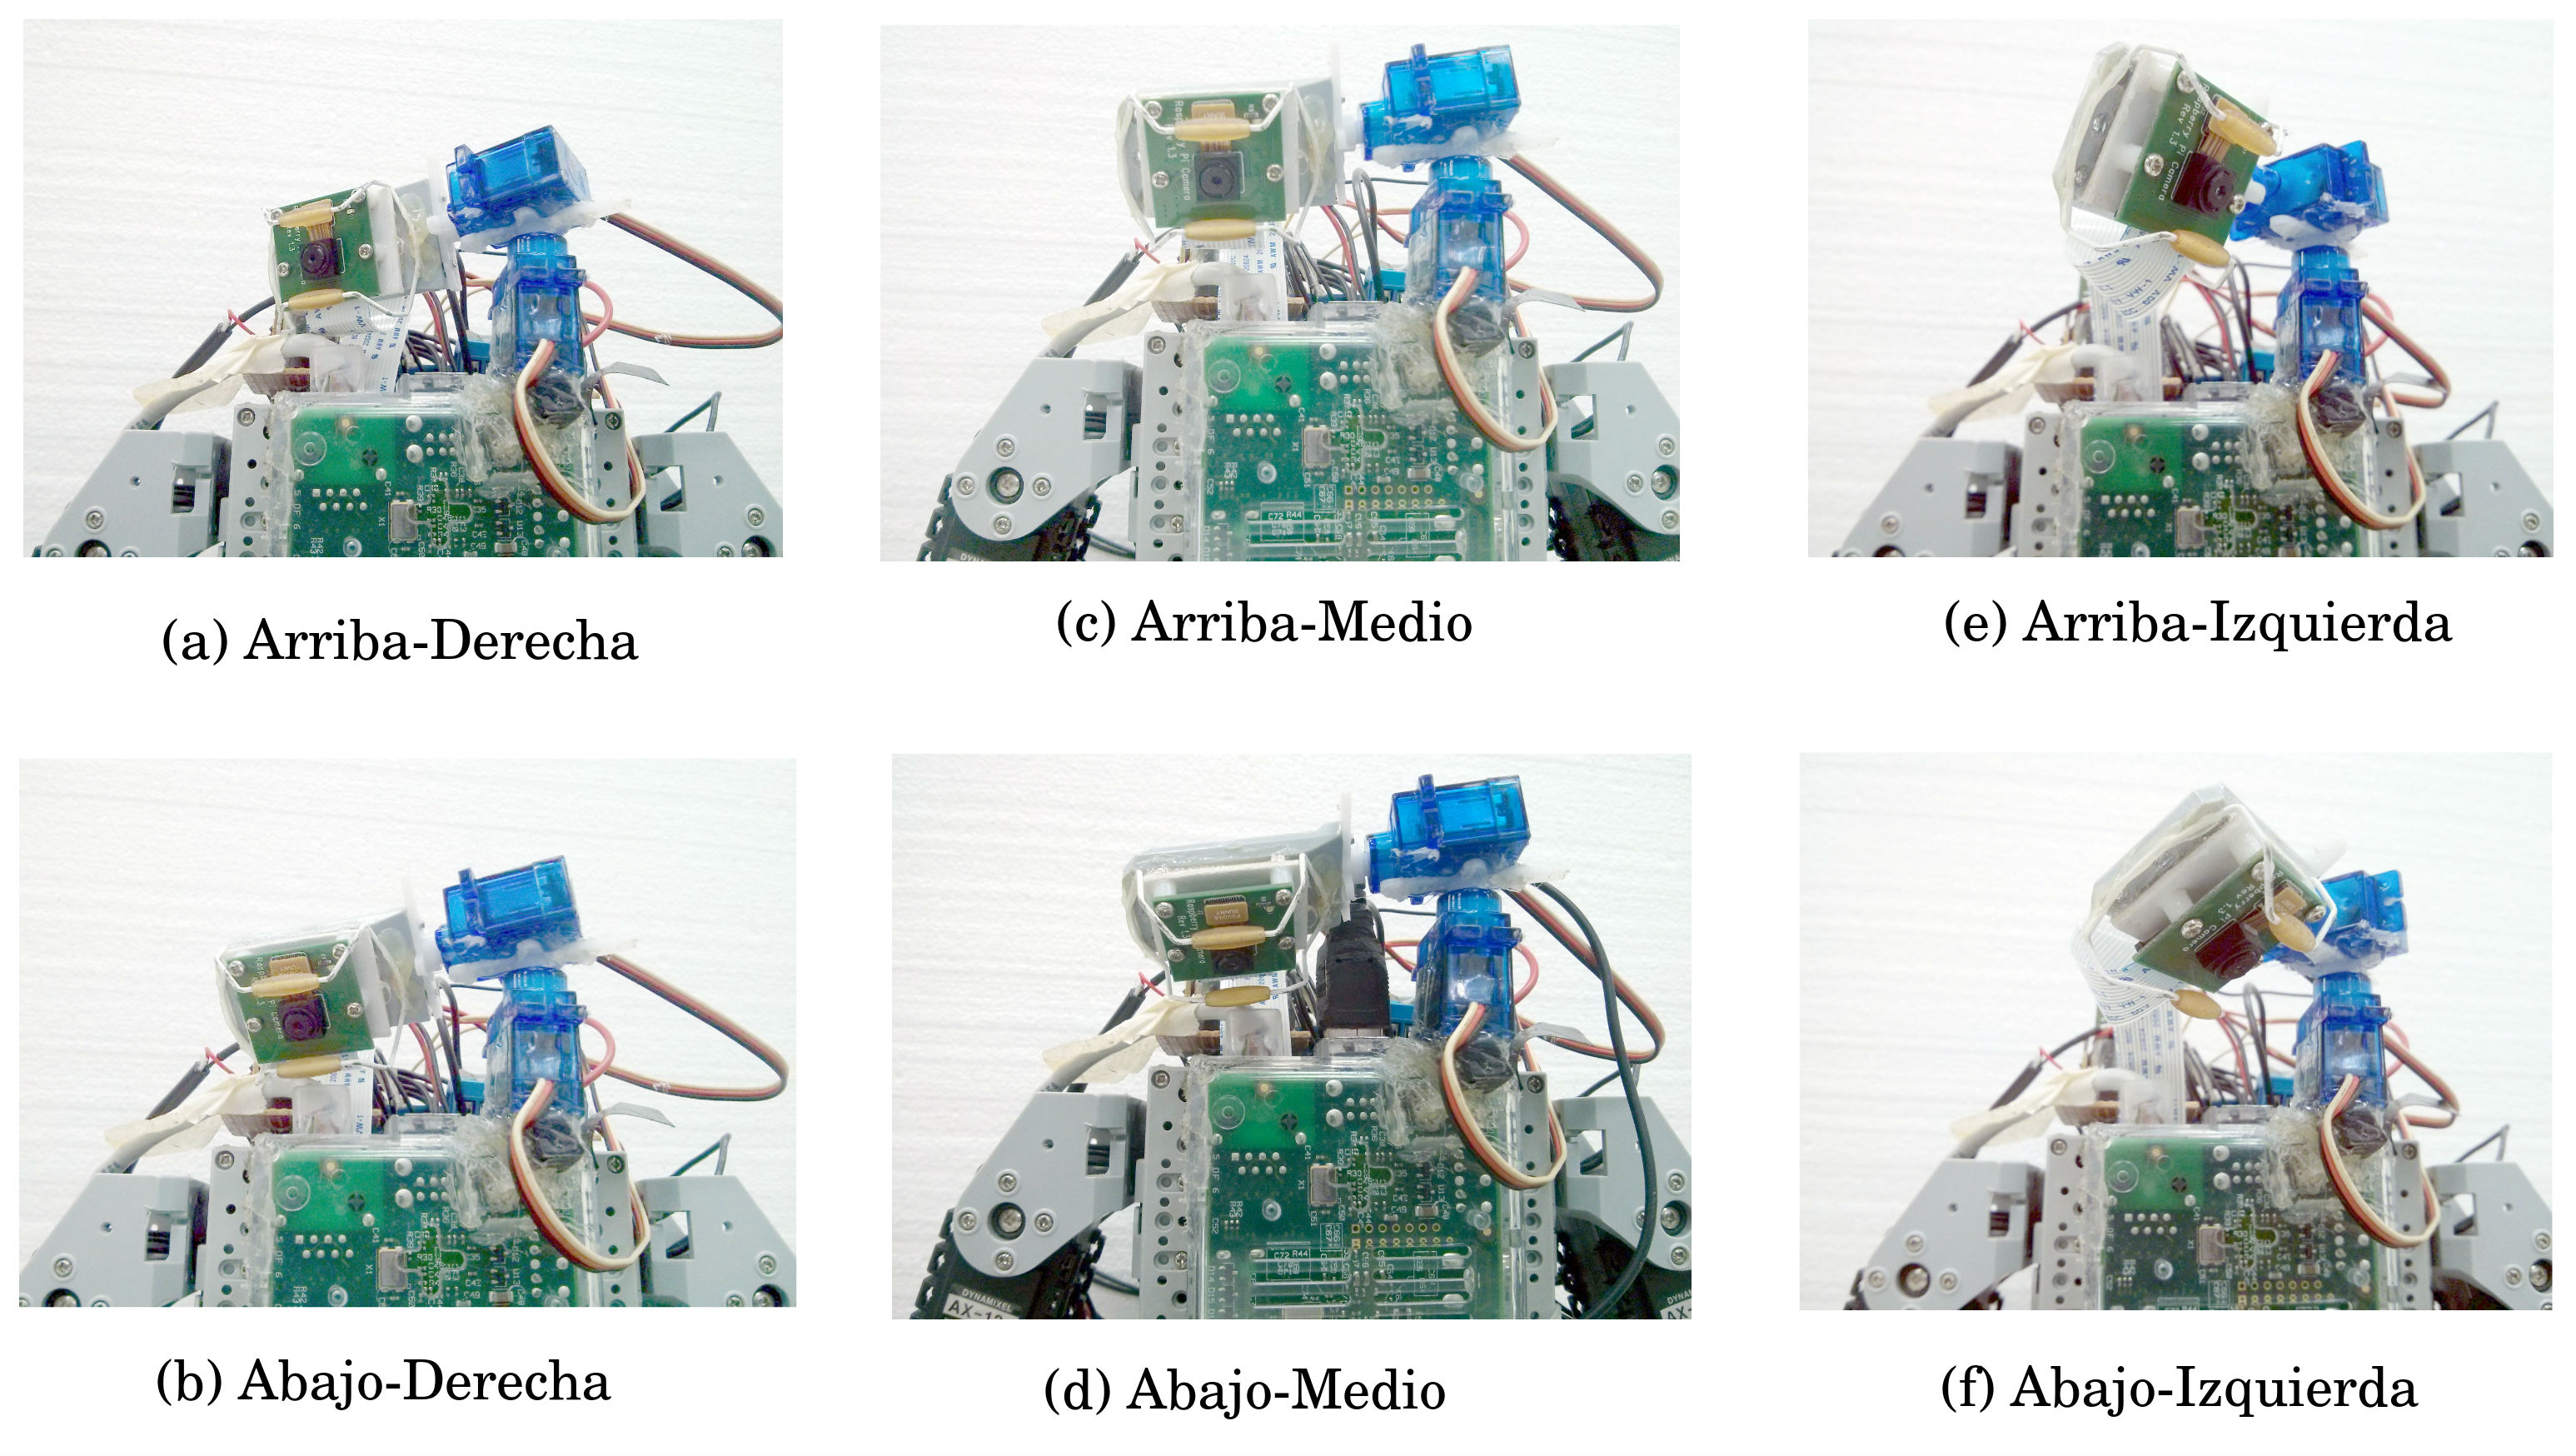
\includegraphics[scale=0.09]{posicionesCamara.jpg} 
\end{figure}
\end{frame}


\begin{frame}
\frametitle{Representaci\'on del mundo}
\begin{figure}[hbtp]
\centering
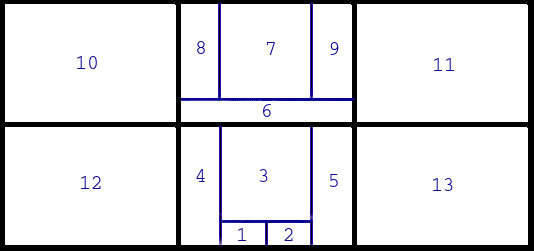
\includegraphics[scale=0.5]{Regiones.jpg} 
\end{figure}
\end{frame}



\begin{frame}
\frametitle{Comunicaci\'on Arbotix-Raspberry Pi}

\begin{itemize}
	\item Herramienta: ROS (Robot Operating System)
	\item Paradigma Cliente/Servidor
	\item Comunicaci\'on bidireccional y s\'incrona
\end{itemize}	

\end{frame}



\begin{frame}
\frametitle{Aprendizaje}

\begin{block}{Motivaci\'on}
\begin{itemize}
	\item Aprendizaje por reforzamiento
	\item Aprendizaje-Q
\end{itemize}
\end{block}	

\begin{block}{Modelo del problema}
\begin{itemize}
	\item Estados
	\item Acciones
	\item Recompensas
\end{itemize}
\end{block}	

\end{frame}


\begin{frame}
\frametitle{Modelo del problema}
\framesubtitle{Estados}
\begin{figure}[hbtp]
\centering
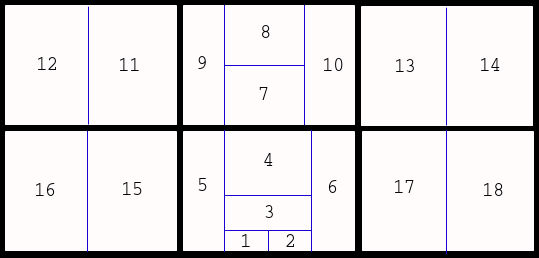
\includegraphics[scale=0.5]{Regiones2.jpg} 
\end{figure}
\end{frame}

\begin{frame}
\frametitle{Modelo del problema}
\framesubtitle{Acciones}

\begin{itemize}
 \item Caminar un paso hacia adelante
 \item Caminar dos pasos hacia adelante
 \item Caminar cuatro pasos hacia adelante
 \item Girar a la izquierda
 \item Girar doble a la izquierda
 \item Girar a la derecha
 \item Girar doble a la derecha
\end{itemize}

\end{frame}


\begin{frame}
\frametitle{Modelo del problema}
\framesubtitle{Recompensas}

\begin{equation}
R(s,a,s') = \dfrac{d(s) - d(s')}{10}
\end{equation}

\begin{figure}[hbtp]
\centering
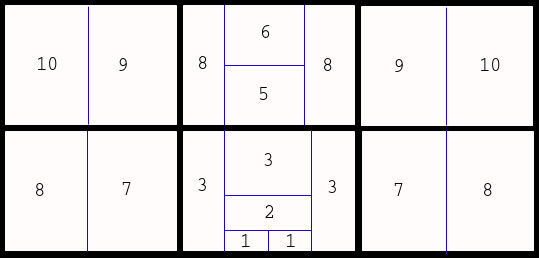
\includegraphics[scale=0.5]{Distancias2.jpg} 
\end{figure}

\end{frame}



\begin{frame}
\frametitle{Aprendizaje}

\begin{block}{Elecci\'on de la acci\'on}
\begin{equation}
 P(a_{i} | s) = \dfrac{k^{Q(s,a_{i})}}{\sum_{j}k^{Q(s,a_{j})}}
\end{equation}
\end{block} 

\begin{block}{Actualizaci\'on de Q(s,a)}
\begin{equation}
Q (s,a) = r + {\gamma\max_{a'}} Q(\delta(s ,a ) , a') 
\end{equation}
\end{block}

\end{frame}




\begin{frame}
\frametitle{Detecci\'on de caidas}
%\framesubtitle{Detecci\'on de ca\'idas}

\begin{itemize}
 \item Velocidad angular (-300,300)
 \item Error estable (-80,100)
\end{itemize}

\begin{figure}[hbtp]
\centering
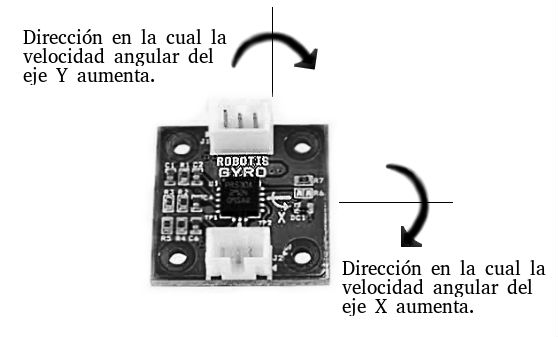
\includegraphics[scale=0.3]{gyroDireccion.jpg} 
\end{figure}

\end{frame}



\begin{frame}
\frametitle{Orientaci\'on al arco}
%\framesubtitle{Orientaci\'on al arco}

\begin{figure}[hbtp]
\centering
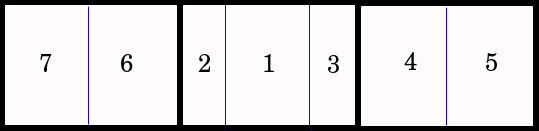
\includegraphics[scale=0.4]{RegionesArco.jpg} 
\end{figure}

\end{frame}


\section{Experimentos y Resultados}


\begin{frame}
\frametitle{Experimentos}
\framesubtitle{Simples}
\begin{block} {De movimiento individual}
Los movimientos individuales son:
\end{block}

\begin{itemize}
\item Caminar un paso hacia adelante 
\item Caminar dos pasos hacia adelante 
\item Caminar cuatro pasos hacia adelante 
\item Girar hacia la derecha 
\item Girar doble a la derecha 
\item Girar hacia la izquierda 
\item Girar doble a la izquierda
\item Patada con la pierna derecha 
\item Patada con la pierna izquierda

\end{itemize}


\end{frame}

\begin{frame}
\frametitle{Experimentos}
\framesubtitle{Simples}
\begin{block} {De movimiento}
Se realizaron 50 ejecuciones de cada movimiento simple
\end{block}

\begin{figure}[scale = 0.1]
\centering
 \resizebox{\textwidth}{!}{%
\begin{tabular}{|c|c|c|c|c|}
\hline 
Movimiento & Cantidad de pruebas & Correctas & Fallidas & Con recuperaci\'on \\ 
\hline 
1 & 50 & 100\% & 0\% & NA \\ 
\hline 
2 & 50 & 98\% & 2\% & 0\% \\ 
\hline 
3 & 50 &  100\% & 0\% & NA \\ 
\hline 
4 & 50 &  100\% & 0\% & NA \\ 
\hline 
5 & 50 &  100\% & 0\% & NA \\ 
\hline 
6 & 50 &  100\% & 0\% & NA \\ 
\hline 
7 & 50 &  100\% & 0\% & NA \\ 
\hline 
8 & 50 &   98\% & 0\% & 2\% \\ 
\hline 
9 & 50 &  100\% & 0\% & NA \\ 
\hline 
\end{tabular} 
}
%\caption{Resultados pruebas individuales de movimiento}
\label{fig:individuales}
\end{figure}

\end{frame}

\begin{frame}
\frametitle{Experimentos}
\framesubtitle{Simples}
\begin{block} {De movimiento compuesto}
Los movimientos elegidos son :
\end{block}

\begin{itemize}

\item Caminar hacia adelante y patear con la pierna derecha 
\item Caminar hacia adelante y patear con la pierna izquierda
\item Caminar hacia adelante, girar hacia la derecha y patear con la pierna derecha
\item Caminar hacia adelante, girar hacia la derecha, patear con la pierna izquierda 
\item Caminar hacia adelante, girar hacia la izquierda y patear con la derecha

\end{itemize}


\end{frame}
\begin{frame}
\frametitle{Experimentos}
\framesubtitle{Simples}

\begin{itemize}


\item Caminar hacia adelante, girar hacia la  izquierda y  patear con la pierna izquierda
\item Girar hacia la izquierda y patear con la pierna derecha
\item Girar hacia la derecha y patear con la izquierda
\item Girar hacia la derecha y patear con la pierna derecha
\item Girar hacia la izquierda y patear con la pierna izquierda


\end{itemize}

\end{frame}
\begin{frame}
\frametitle{Experimentos}
\framesubtitle{Simples}
\begin{block} {De movimiento compuesto}
Se realizaron 30 ejecuciones de cada movimiento compuesto
\end{block}

\begin{figure}[scale = 0.1]
\centering
 \resizebox{\textwidth}{!}{%
\begin{tabular}{|c|c|c|c|c|}
\hline 
Combinaci\'on & Cantidad de pruebas & Correctas & Fallidas & Con recuperaci\'on \\ 
\hline 
1 & 30 & 96.7\% & 3.3\% & 0\% \\ 
\hline 
2 & 30 & 100\% & 0\% & NA \\ 
\hline 
3 & 30 & 100\% & 0\% & NA \\ 
\hline 
4 & 30 & 100\% & 0\% & NA \\ 
\hline 
5 & 30 & 96.7\% & 3.3\% & 0\% \\ 
\hline 
6 & 30 & 100\% & 0\% & NA \\ 
\hline 
7 & 30 & 100\% & 0\% & NA \\ 
\hline 
8 & 30 & 100\% & 0\% & NA \\ 
\hline 
9 & 30 & 100\% & 0\% & NA \\ 
\hline 
10 & 30 & 100\% & 0\% & NA \\ 
\hline 
\end{tabular} 
}
\end{figure}

\end{frame}
\begin{frame}
\frametitle{Experimentos}
\framesubtitle{Simples}
\begin{block} {De movimiento compuesto}
Se realizaron 50 ejecuciones de cada prueba de enfoque
\end{block}

\begin{figure}[scale = 0.1]
\centering
 %\resizebox{\textwidth}{!}{%
\begin{tabular}{|c|c|c|}
 \hline 
  & Cantidad de Pruebas & Correctas \\ 
 \hline 
 A 50 cm & 50 & 100\% \\ 
 \hline 
 A 80 cm & 50 & 100\% \\ 
 \hline 
 No pelota & 50 & 100\% \\ 
  \hline 

 \end{tabular}  
%}
\end{figure}

\end{frame}

%\end{frame}


\begin{frame}
\frametitle{Experimentos}
\framesubtitle{Compuestos}
\begin{block} {Comportamiento integrados}
\begin{itemize}
\item Caso I :Pelota a los pies de Junny
\item Caso II: Pelota a 50 cm en linea recta 
\item Caso III: Pelota 50 cm en linea recta y 50 cm a la izquierda
\item Caso IV: Pelota 50 cm en linea recta y 50 cm a la derecha
\end{itemize}
\end{block}

\begin{figure}[scale = 0.1]
\centering
 \resizebox{\textwidth}{!}{%
\begin{tabular}{|p{3cm}|p{2cm}|c|p{2cm}|c|p{2cm}|}
\hline 
& Cantidad de 
pruebas realizadas & Correctas & Con fallas recuperadas & Fallidas & Tiempo Promedio \\ 
%\hline 
%Subconjunto de combinadas & 300 & 96\% & 4\% & NA & NA \\ 
\hline 
Caso I & 10 & 90\% & 10\% & 0\% & 30 s \\ 
\hline 
Caso II & 10 & 70\% & 10\% & 20\% & 2m 12s \\ 
\hline 
Caso III & 10 & 80\% & 0\% & 20\% & 3m 29s \\ 
\hline 
Caso IV & 10 & 90\% & 0\% & 10\% & 4m 48s \\ 
\hline 
\end{tabular} 
}
\end{figure}

\end{frame}
\begin{frame}
  \frametitle{Experimentos}
  \framesubtitle{Aprendizaje}
  \begin{block}{Ajuste}
  \begin{itemize}
  \item Pruebas con variaciones en los parametros
  \item $K = 3   \gamma = 0.1$ con 
  el 100\% de aciertos
	
  \end{itemize}
		\end{block}

\begin{figure}
\centering
\begin{tabular}{|c|c|c|c|}
\hline 
& Cantidad & Correctas & Fallidas \\ 
\hline 
$K = 1  \gamma = 0.1$ & 20 & 80\% & 20\% \\ 
\hline 
$K = 2  \gamma = 0.1$ & 20 & 80\% & 20\% \\ 
\hline 
$K = 2  \gamma = 0.7$ & 20 & 60\% & 40\% \\ 
\hline 
$K = 3  \gamma = 0.1$ & 20 & 90\% & 10\% \\ 
\hline 
$K = 3  \gamma = 0.7$ & 20 & 80\% & 20\% \\ 
\hline 
$K = 5  \gamma = 0.1$ & 20 & 80\% & 20\% \\ 
\hline  
$K = 5  \gamma = 0.7$ & 20 & 70\% & 30\% \\ 
\hline 

\end{tabular} 

\caption{Resultados de los distintos par\'ametros con aprendizaje}
\label{tabla:entramientos}


\end{figure}

\end{frame}

\begin{frame}
  \frametitle{Experimentos}
  \framesubtitle{Aprendizaje}
  \begin{block}{Comparaci\'on}
	Se compararon las pruebas con los casos de pruebas integradas
\end{block}

\begin{figure}
\centering
\begin{tabular}{|c|c|c|c|}
\hline  & Caso II & Caso III & Caso IV \\ 
\hline 
Correctas con aprendizaje & 100\% & 100\% & 100\% \\ 
\hline 
Correctas sin aprendizaje & 70\% & 80\% & 90\% \\ 
\hline 
Fallidas con aprendizaje & 0\% & 0\% & 0\% \\ 
\hline 
Fallidas sin aprendizaje & 20\% & 20\% & 10\% \\ 
\hline 
Recuperadas con aprendizaje & NA & NA & NA \\ 
\hline 
Recuperadas sin aprendizaje & 10\% & 0\% & 0\% \\ 
\hline 
Tiempo promedio con aprendizaje & 2m 35 s & 5m 38s & 4m 14s \\ 
\hline 
Tiempo promedio sin aprendizaje & 2m 12s & 3m 29 s & 4m 48s \\
\hline
%\caption{Cada prueba tiene un numero de corridas de 10}
\end{tabular} 
\caption{Comparaci\'on de movimientos predeterminados y aprendizaje}
\label{tabla:comparacion}

\end{figure}

\end{frame}



\begin{frame}
\frametitle{Experimentos}
\begin{block}{Completos}
Los experimentos con el comportamiento completo incluyendo orientaci\'on al arco y el aprendizaje por reforzamiento con un resultado de 40 \% de fallo, 6.6 \% Tiros al arco y 53 \% Goles marcados
\end{block}


\end{frame}

\section{Conclusiones}

\begin{frame}
\frametitle{Conclusiones}
 \begin{block}{Puntos relevantes}
  \begin{itemize}
\item 99.6 \% de aciertos en simples
\item 96 \% en compuestos realizados correctamente
\item 100 \% en la detecci\'on de la pelota
\item 70 \% en caso II y 90\% en casos I y IV
\item 100 \% en aprendizaje y un 0.72 en eficiencia
\item 53 \% con orientaci\'on al arco
\item Integraci\'on de todos los componentes
\item Incursi\'on en rob\'otica (humanoide)
\item Econ\'omico
  \end{itemize}

 \end{block}

\end{frame}

\section{Futuros Trabajos}
\begin{frame}
\frametitle{Trabajos Futuros }
\begin{block}{}
\begin{itemize}
\item Aumentar acciones y regiones
\item Caderas
\item Motores distintos
\item Aprendizaje para:
\begin{itemize}
	\item Detecci\'on de pelota
	\item Predicci\'on 
	\item Tipo de patada
	\item Compa\~nero
\end{itemize}
\end{itemize}
\end{block}
\end{frame}
\begin{frame}

\LARGE{PREGUNTAS}
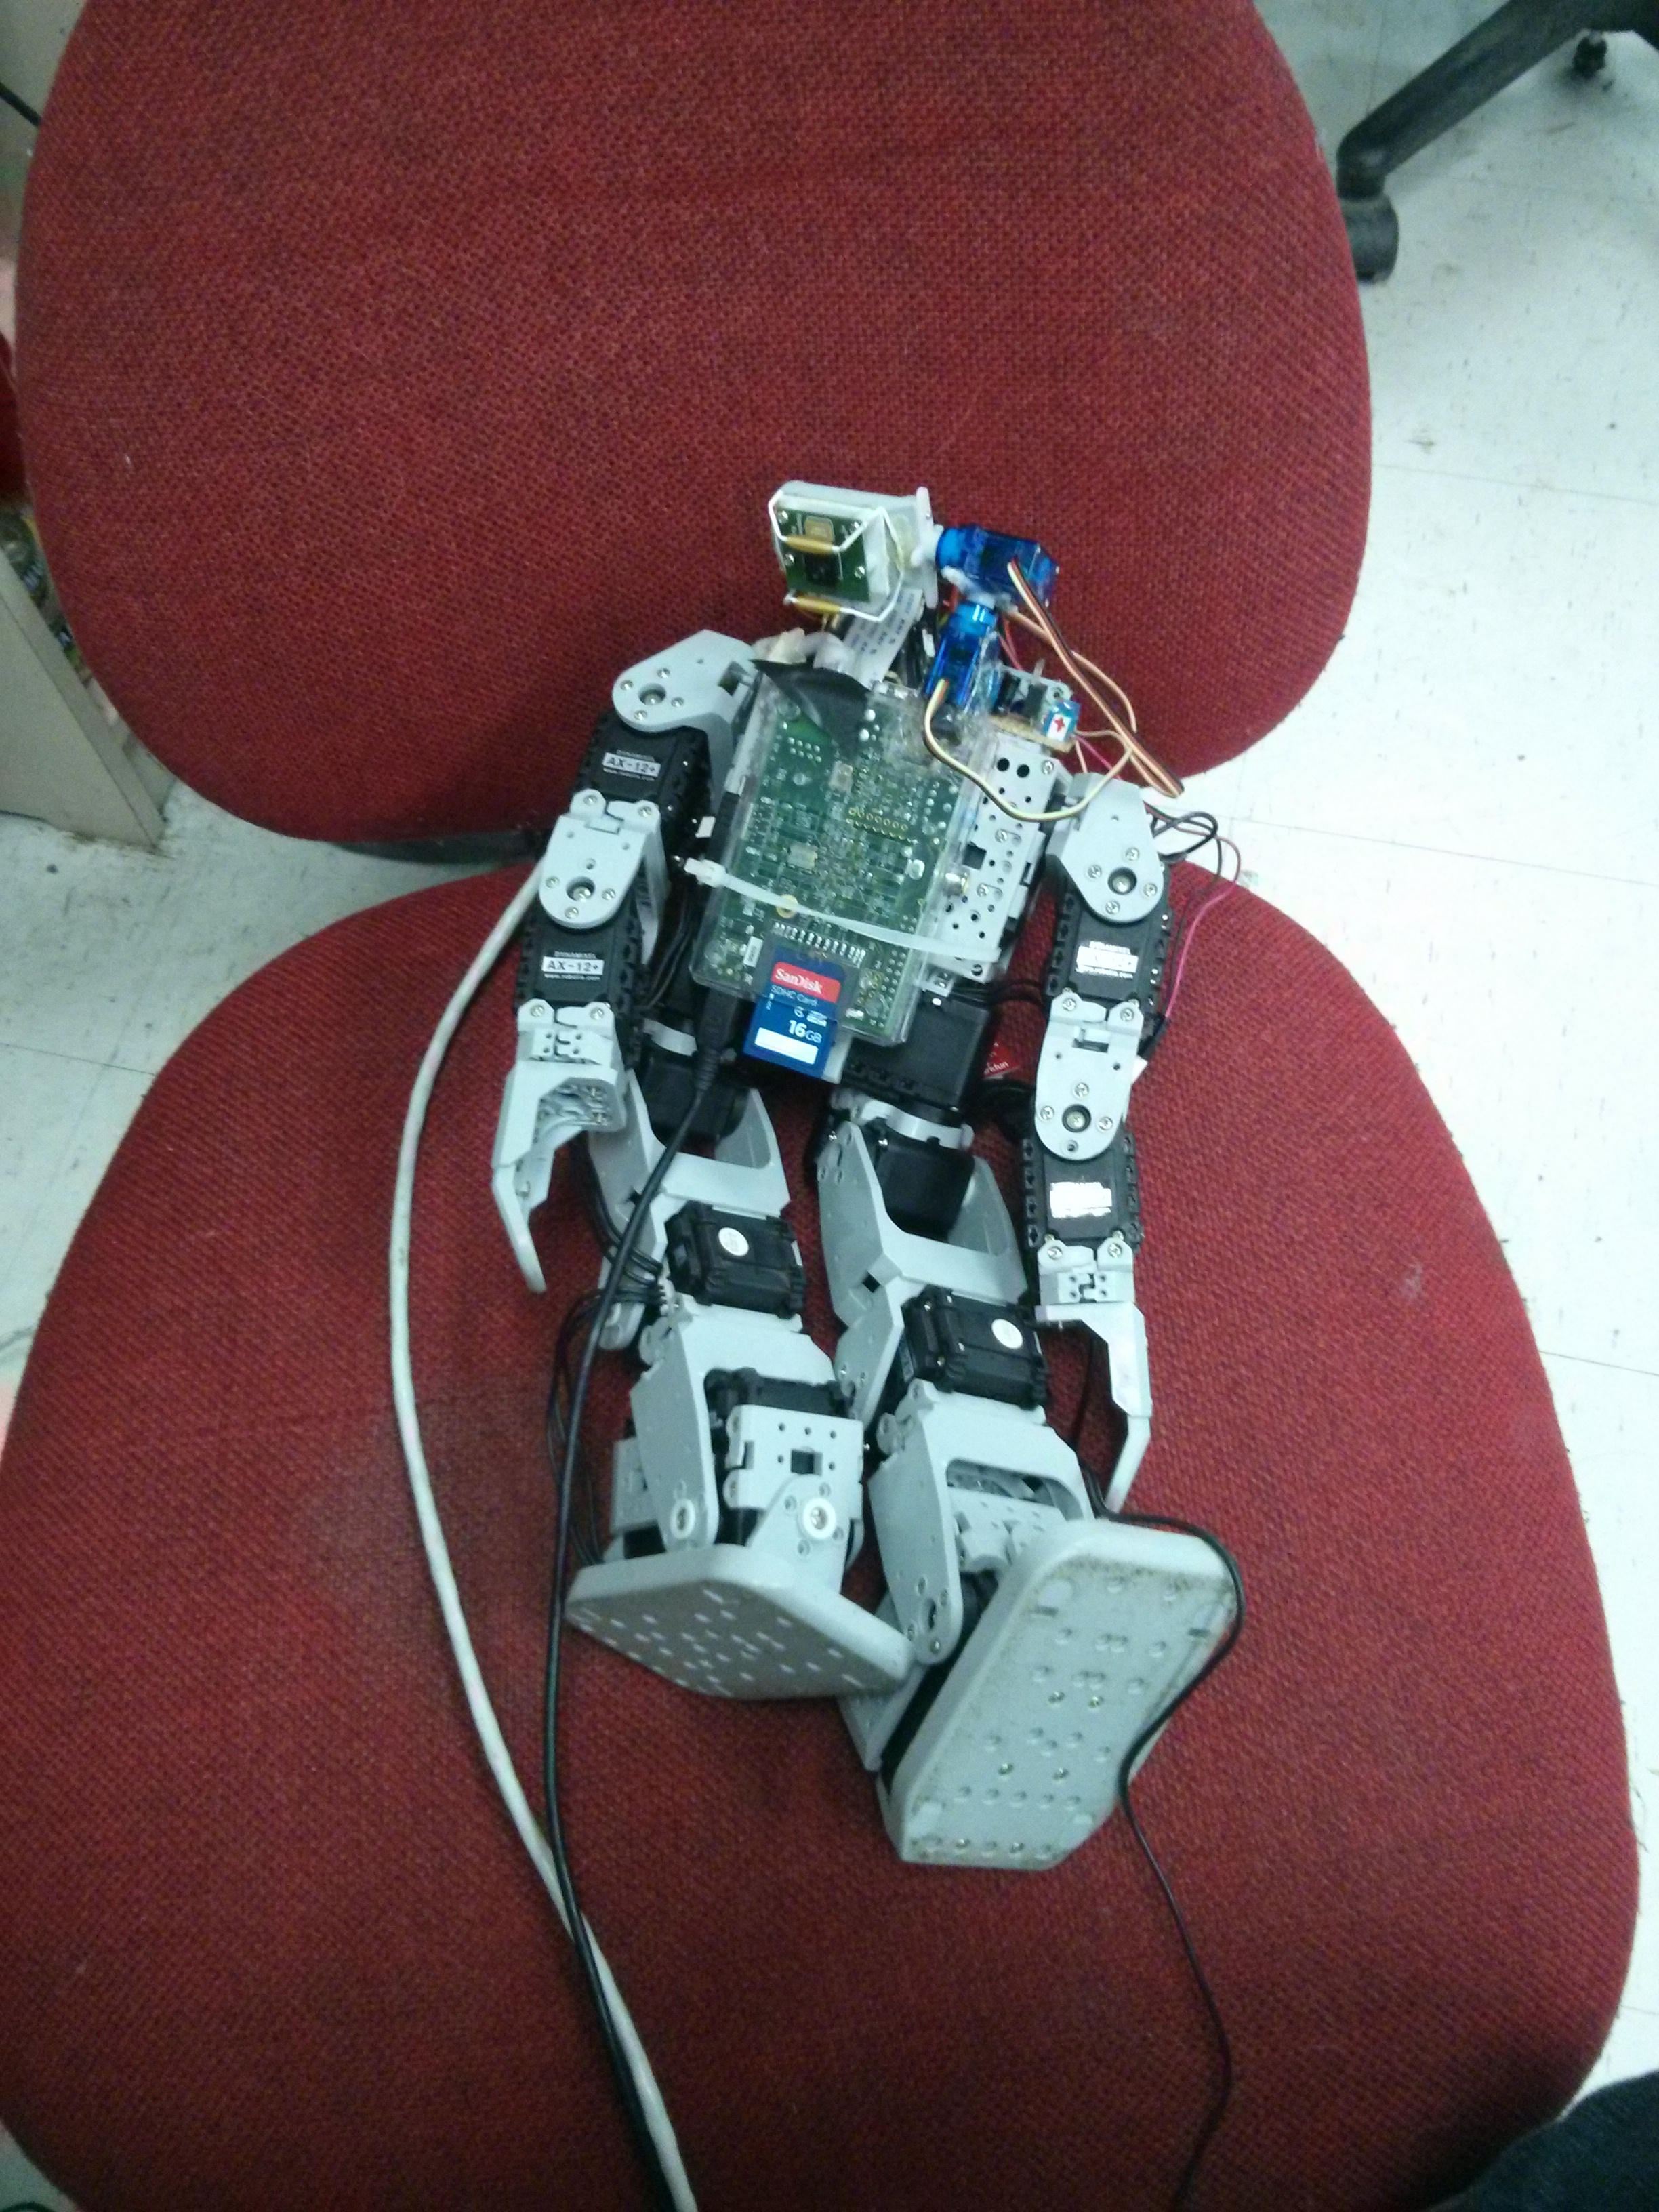
\includegraphics[scale=0.05]{tirolesa}
\end{frame}
\end{document}